\begin{tikzpicture}[>=stealth,scale=.8,
	setts/.style={color=black,very thick, ->},
	cross/.style={color=black,very thick}]

	\node at (0,0) {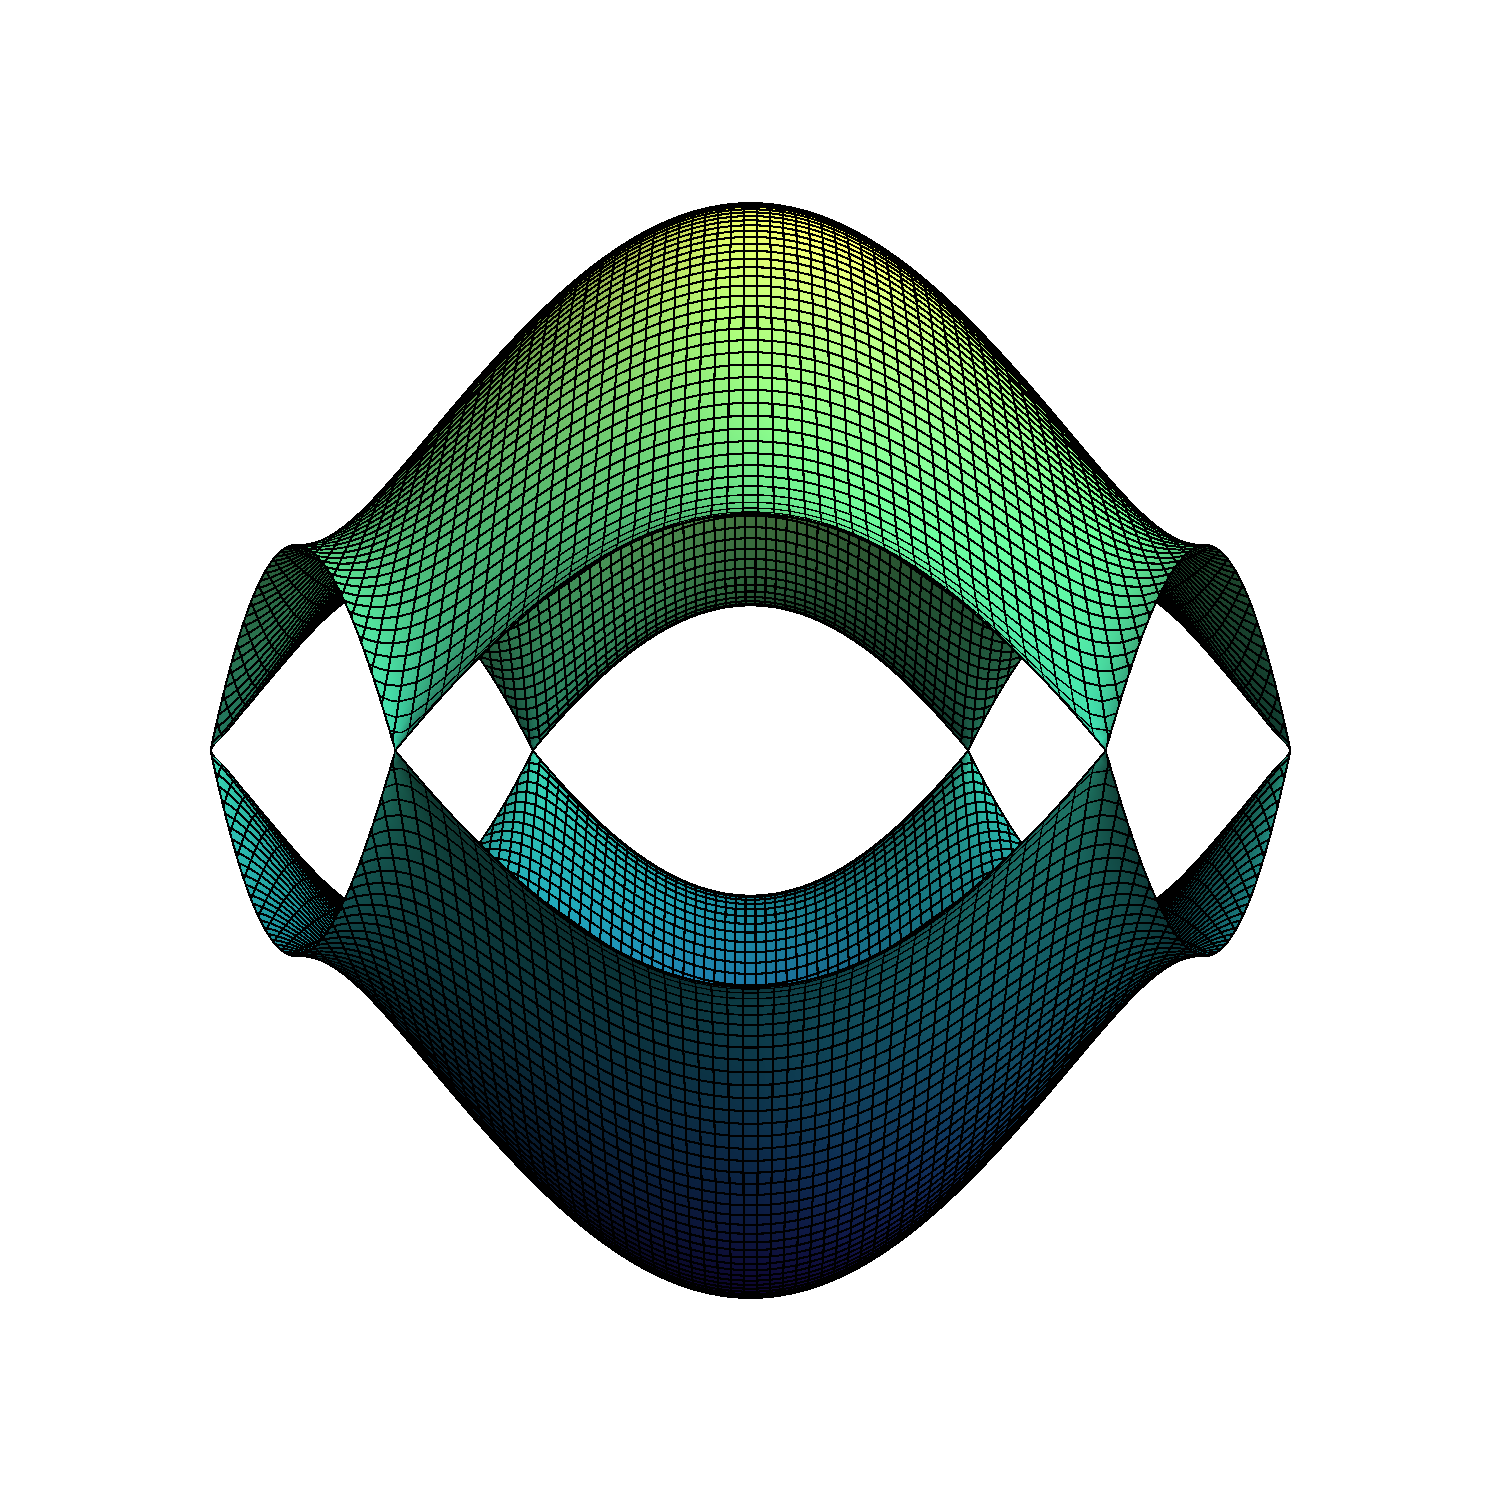
\includegraphics{Figs_TightBinding/bandstructure_thesis.png}};
	\node at (-5,0)[anchor=center]{$\bm{K}$};
	\node at ( 5,0)[anchor=center]{$\bm{K'}$};

	% Coordinate axis
	\begin{scope}[xshift=-6cm,yshift=-6cm]
		\draw[setts] (0,0) -- (0,12 cm) node [anchor=south east] {$E$};
		\draw[setts] (0,0) -- (12 cm,0) node [anchor=north west] {$k_x$};
		% The out of plane axis
		\draw[cross] (-3 pt, -3 pt) -- ( 3 pt, 3 pt);
		\draw[cross] (-3 pt,  3 pt) -- ( 3 pt,-3 pt);
		\node at (0,0)[anchor=north east] {$k_y$};
		% \draw[fill=black,color=black] (0,0) circle[radius=3pt] node[anchor=north east] {$k_y$};
	\end{scope}
\end{tikzpicture}